\documentclass[a4paper]{jarticle}
\usepackage{comment}
\usepackage{slashbox}
\usepackage{listings,jlisting}
\usepackage[dvipdfmx]{graphicx}
\usepackage[top=20truemm,bottom=20truemm,left=20truemm,right=20truemm]{geometry}
\title{計算機工学実験A課題3レポート}
\author{学生番号 氏名}
\date{2016/11/24}
\lstset{%
	basicstyle={\small},%
	tabsize=8,
	identifierstyle={\small},%
	commentstyle={\small\itshape},%
	keywordstyle={\small\bfseries},%
	ndkeywordstyle={\small},%
	stringstyle={\small\ttfamily},
	frame={tb},
	breaklines=true,
	columns=[1]{fullflexible},%
	numbers=left,%
	xrightmargin=0zw,%
	xleftmargin=3zw,%
	numberstyle={\scriptsize},%
	stepnumber=1,
	numbersep=1zw,%
	lineskip=-0.5ex,%
	keepspaces=true,
	showstringspaces=false
}
\begin{document}
\maketitle
\section{実験の総括的な目的}
\section{各課題の結果}
\subsection{課題1}
\subsubsection{目的}
$iSW[0]$から$iSW[7]$までのスイッチ入力を$oLEDR[0]$から$oLEDR[7]$までに素通しする配線を$Verilog$で記述して、動作を確認する。
\subsubsection{道のり}
トップモジュールに以下のようなコードを追加し、コンパイルしてハードウェアに流し込み、動作を確認した。
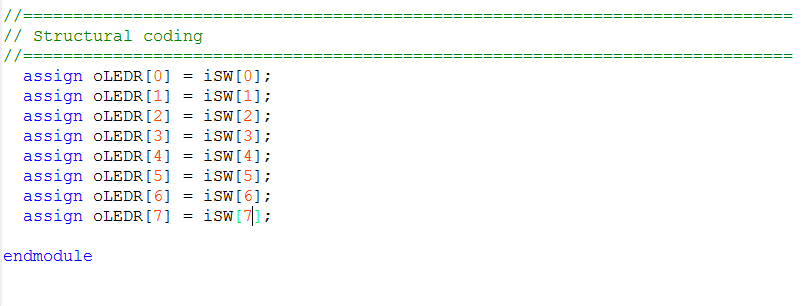
\includegraphics[width=15cm]{work1/1.PNG}
\subsubsection{結果}
意図したとおりに、以下の真理値表に従い、$iSW[0]$から$iSW[7]$までのON,OFFにに対応して、$oLEDR[0]$から$oLEDR[7]$までがそれぞれ光ったり光らなかったりした。
\begin{table}[!h]
	\begin{center}
		\begin{tabular}{c}
			\begin{minipage}{0.5\hsize}
				\begin{center}
					\caption{動作の真理値表1}
					\label{Work1TruthTable1}
					\begin{tabular}{|c|c|}
						\hline
						$iSW[0]$	&$oLEDR[0]$\\	\hline\hline
						$0$		&$0$\\		\hline
						$1$		&$1$\\		\hline
					\end{tabular}
				\end{center}
			\end{minipage}
			\begin{minipage}{0.5\hsize}
				\begin{center}
					\caption{動作の真理値表2}
					\label{Work1TruthTable2}
					\begin{tabular}{|c|c|}
						\hline
						$iSW[1]$	&$oLEDR[1]$\\	\hline\hline
						$0$		&$0$\\		\hline
						$1$		&$1$\\		\hline
					\end{tabular}
				\end{center}
			\end{minipage}
		\end{tabular}
	\end{center}
\end{table}
\begin{table}[!h]
	\begin{center}
		\begin{tabular}{c}
			\begin{minipage}{0.5\hsize}
				\begin{center}
					\caption{動作の真理値表3}
					\label{Work1TruthTable3}
					\begin{tabular}{|c|c|}
						\hline
						$iSW[2]$	&$oLEDR[2]$\\	\hline\hline
						$0$		&$0$\\		\hline
						$1$		&$1$\\		\hline
					\end{tabular}
				\end{center}
			\end{minipage}
			\begin{minipage}{0.5\hsize}
				\begin{center}
					\caption{動作の真理値表4}
					\label{Work1TruthTable4}
					\begin{tabular}{|c|c|}
						\hline
						$iSW[3]$	&$oLEDR[3]$\\	\hline\hline
						$0$		&$0$\\		\hline
						$1$		&$1$\\		\hline
					\end{tabular}
				\end{center}
			\end{minipage}
		\end{tabular}
	\end{center}
\end{table}
\begin{table}[!h]
	\begin{center}
		\begin{tabular}{c}
			\begin{minipage}{0.5\hsize}
				\begin{center}
					\caption{動作の真理値表5}
					\label{Work1TruthTable5}
					\begin{tabular}{|c|c|}
						\hline
						$iSW[4]$	&$oLEDR[4]$\\	\hline\hline
						$0$		&$0$\\		\hline
						$1$		&$1$\\		\hline
					\end{tabular}
				\end{center}
			\end{minipage}
			\begin{minipage}{0.5\hsize}
				\begin{center}
					\caption{動作の真理値表6}
					\label{Work2TruthTable6}
					\begin{tabular}{|c|c|}
						\hline
						$iSW[5]$	&$oLEDR[5]$\\	\hline\hline
						$0$		&$0$\\		\hline
						$1$		&$1$\\		\hline
					\end{tabular}
				\end{center}
			\end{minipage}
		\end{tabular}
	\end{center}
\end{table}
\subsubsection{考察}
ハードウェア上の入力、出力にそれぞれつながっている$iSW[x]$と$oLEDR[x]$を単純に繋げ、とても単純な回路だが、正しくハードウェア上で実行することが出来た。$System Verilog$のコードを見ただけではわかりにくくても、実際にハードウェア上で実行することによってコードの意味をより理解できるだろうと感じた。
\subsection{課題2}
\subsubsection{目的}
ビット毎の演算子$NOT,AND,OR,XOR$を試す論理回路を$Verilog$で記述して、働きを確認する。
\subsubsection{道のり}
まず、$DE2\_TOP.sv$をコピーペーストし、その中で定義されているモジュール$DE2\_TOP$に、ビット毎の演算子$NOT,AND,OR,XOR$を試す論理回路を定義したソースコード\ref{Work2TOP}を作成した。
\lstinputlisting[caption=$DE2\_TOP.sv$,label=Work2TOP]{work2/DE2_TOP.sv}
その後、これをコンパイルしてハードウェアに流し込み、動作を確認した。
\subsubsection{結果}
実際のハードウェア上では、作成した回路は以下の表\ref{Work2NotGateTruthTable},\ref{Work2AndGateTruthTable},\ref{Work2OrGateTruthTable},\ref{Work2XorGateTruthTable}の真理値表のように動作した。
\begin{table}[!h]
	\begin{center}
		\caption{$NOT$回路の真理値表}
		\label{Work2NotGateTruthTable}
		\begin{tabular}{|c|c|c|}
			\hline
			$iSW \left[ 0 \right]$	&$oLEDR \left[ 0 \right]$	&$oLEDR \left[ 1 \right]$\\	\hline\hline
			$0$			&$0$				&$1$\\				\hline
			$1$			&$1$				&$0$\\				\hline
		\end{tabular}
	\end{center}
\end{table}
\begin{table}[!h]
	\begin{center}
		\caption{$AND$回路の真理値表}
		\label{Work2AndGateTruthTable}
		\begin{tabular}{|c|c|c|c|c|}
			\hline
			$iSW \left[ 1 \right]$	&$iSW \left[ 2 \right]$	&$oLEDR \left[ 2 \right]$	&$oLEDR \left[ 3 \right]$	&$oLEDR \left[ 4 \right]$\\	\hline\hline
			$0$			&$0$			&$0$				&$0$				&$0$\\				\hline
			$0$			&$1$			&$0$				&$1$				&$0$\\				\hline
			$1$			&$0$			&$1$				&$0$				&$0$\\				\hline
			$1$			&$0$			&$1$				&$1$				&$1$\\				\hline
		\end{tabular}
	\end{center}
\end{table}
\begin{table}[!h]
	\begin{center}
		\caption{$OR$回路の真理値表}
		\label{Work2OrGateTruthTable}
		\begin{tabular}{|c|c|c|c|c|}
			\hline
			$iSW \left[ 3 \right]$	&$iSW \left[ 4 \right]$	&$oLEDR \left[ 5 \right]$	&$oLEDR \left[ 6 \right]$	&$oLEDR \left[ 7 \right]$\\	\hline\hline
			$0$			&$0$			&$0$				&$0$				&$0$\\				\hline
			$0$			&$1$			&$0$				&$1$				&$1$\\				\hline
			$1$			&$0$			&$1$				&$0$				&$1$\\				\hline
			$1$			&$0$			&$1$				&$1$				&$1$\\				\hline
		\end{tabular}
	\end{center}
\end{table}
\begin{table}[!h]
	\begin{center}
		\caption{$XOR$回路の真理値表}
		\label{Work2XorGateTruthTable}
		\begin{tabular}{|c|c|c|c|c|}
			\hline
			$iSW \left[ 5 \right]$	&$iSW \left[ 6 \right]$	&$oLEDR \left[ 8 \right]$	&$oLEDR \left[ 9 \right]$	&$oLEDR \left[ 10 \right]$\\	\hline\hline
			$0$			&$0$			&$0$				&$0$				&$0$\\				\hline
			$0$			&$1$			&$0$				&$1$				&$1$\\				\hline
			$1$			&$0$			&$1$				&$0$				&$1$\\				\hline
			$1$			&$0$			&$1$				&$1$				&$0$\\				\hline
		\end{tabular}
	\end{center}
\end{table}
\subsubsection{考察}
モジュール$DE2\_TOP$に単純な回路を組み込むことによって、$Verilog$の基本的な論理演算子が正常に動作することを確認できた。単にスイッチからの配線を論理ゲートに通してからLEDにつなぐのではなく、スイッチからの配線を別のLEDにそのままつないだものも用意することによって、ハードウェア上で実行したときの結果が分かりやすかった。
\subsection{課題3}
\subsubsection{目的}
算術の演算子$PLUS,MINUS$を$Verilog$で記述して、動きを確認する。
\subsubsection{道のり}
トップモジュールを以下のソースコード\ref{Work3TOP}のように編集して、加算と減算の回路を実現した。そしてコンパイルしてハードウェアに流し込み、動作を確認した。
\lstinputlisting[caption=$DE2\_TOP.sv$,label=Work3TOP]{work3/DE2_TOP.sv}
\subsubsection{結果}
意図したとおりに、$oLEDR[3:0]$は$iSW[3:0]$と$iSW[7:4]$の和のとおりに光り、$oLEDR[7:4]$は$iSW[11:8]$と$iSW[15:12]$の差のとおりに光った。
\subsubsection{考察}
$Verilog$では、$AND$や$OR$のような論理ゲートだけではなく、加算や減算といった演算を実現できる演算子も用意されていることを知った。このような演算子が用意されていることによって、複雑な回路設計がより楽になるだろうと感じた。
\subsection{課題4}
\subsubsection{目的}
半加算器を実現するモジュール$\left( halfadder.sv \right)$を定義し、スイッチや$LED$を接続して試す。
\subsubsection{道のり}
まず、以下の画像に示したようにモジュール$halfadder.sv$を定義した。\\
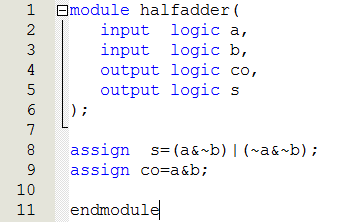
\includegraphics[width=5cm]{work4/4-2.PNG}\\
次に、以下の画像のように、$halfadder$のトップモジュールに組み込んだ。\\
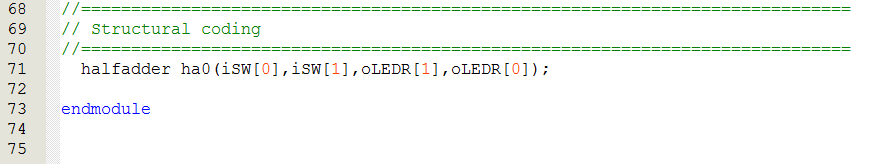
\includegraphics[width=15cm]{work4/4-1.PNG}
\subsubsection{結果}
意図したとおりに、$iSW[0]$と$iSW[1]$の和が$oLEDR[0]$に表示され、繰り上がりが$oLEDR[1]$に表示された。
\subsubsection{考察}
半加算器のモジュールを定義し、トップモジュールに組み込んでその動作を確認した。既成のモジュールをほかのモジュールに組み込んでより複雑な回路を設計する階層設計という方法を知った。階層設計によって、複雑で大きな回路も、単純な回路に分割してモジュールを作成し、そのモジュールを上位のモジュールで繋げることで設計しやすくなるだろうと感じた。
\subsection{課題5}
\subsubsection{目的}
1ビットの全加算器を実現するモジュール$fulladder$を設計し、トップモジュールに組み込んで試す。
\subsubsection{道のり}
まず、1ビットの全加算器を実現するモジュールを、ソースコード\ref{Work5FullAdder}で定義した。ここでは、単純にassignで配線をつないだモジュール$fulladder$と、課題4で作成した半加算器のモジュール$halfadder$を二つ使用した$fulladderUsingHalfadder$を作成した。
\lstinputlisting[caption=$fulladder.sv$,label=Work5FullAdder]{work5/fulladder.sv}
次に、ソースコード\ref{Work5TOP}にあるように、ソースコード\ref{Work5FullAdder}で定義した二つの全加算器をトップモジュールに組み込み、コンパイルしてハードウェアに流し込み動作を確認した。
\lstinputlisting[caption=$DE2\_TOP.sv$,label=Work5TOP]{work5/DE2_TOP.sv}
\subsubsection{結果}
実際のハードウェア上では、作成した回路は以下の表\ref{Work5FullAdderTruthTable},\ref{Work5FullAdderUsingHalfAdderTruthTable}の真理値表のように動作した。
\begin{table}[!h]
	\begin{center}
		\caption{モジュール$fulladder$の動作の真理値表}
		\label{Work5FullAdderTruthTable}
		\begin{tabular}{|c|c|c|c|c|}
			\hline
			$iSW \left[ 0 \right]$	&$iSW \left[ 1 \right]$	&$iSW \left[ 2 \right]$	&$oLEDR \left[ 0 \right]$	&$oLEDR \left[ 1 \right]$\\	\hline\hline
			$a$			&$b$			&$c$			&$co$				&$s$\\				\hline\hline
			$0$			&$0$			&$0$			&$0$				&$0$\\				\hline
			$0$			&$0$			&$1$			&$0$				&$1$\\				\hline
			$0$			&$1$			&$0$			&$0$				&$1$\\				\hline
			$0$			&$1$			&$1$			&$1$				&$0$\\				\hline
			$1$			&$0$			&$0$			&$0$				&$1$\\				\hline
			$1$			&$0$			&$1$			&$1$				&$0$\\				\hline
			$1$			&$1$			&$0$			&$1$				&$0$\\				\hline
			$1$			&$1$			&$1$			&$1$				&$1$\\				\hline
		\end{tabular}
	\end{center}
\end{table}
\begin{table}[!h]
	\begin{center}
		\caption{モジュール$fulladderUsingHalfadder$の動作の真理値表}
		\label{Work5FullAdderUsingHalfAdderTruthTable}
		\begin{tabular}{|c|c|c|c|c|}
			\hline
			$iSW \left[ 3 \right]$	&$iSW \left[ 4 \right]$	&$iSW \left[ 5 \right]$	&$oLEDR \left[ 2 \right]$	&$oLEDR \left[ 3 \right]$\\	\hline\hline
			$a$			&$b$			&$c$			&$co$				&$s$\\				\hline\hline
			$0$			&$0$			&$0$			&$0$				&$0$\\				\hline
			$0$			&$0$			&$1$			&$0$				&$1$\\				\hline
			$0$			&$1$			&$0$			&$0$				&$1$\\				\hline
			$0$			&$1$			&$1$			&$1$				&$0$\\				\hline
			$1$			&$0$			&$0$			&$0$				&$1$\\				\hline
			$1$			&$0$			&$1$			&$1$				&$0$\\				\hline
			$1$			&$1$			&$0$			&$1$				&$0$\\				\hline
			$1$			&$1$			&$1$			&$1$				&$1$\\				\hline
		\end{tabular}
	\end{center}
\end{table}
\subsubsection{考察}
今回は単純に入力から出力へと配線をつなぐ方法と、半加算器二つを使う方法で同じ動作をする全加算器を作成した。前者の方法は、真理値表通りに作られているので全加算器であることが分かりやすいが、後者の方は、これが全加算器であるといわれなければこれがどんな働きをするのか直感的にはわからないだろうと思った。また、二つの全加算器をトップモジュールに同時に組み込むことで、動作を確認するときに二つが同じ結果を出しているかどうか確認しやすかった。
\subsection{課題6}
\subsubsection{目的}
以下のソースコード\ref{Work6Source}に対応する回路図を書く。
\begin{lstlisting}[caption=信号を束ねる例,label=Work6Source]
assign oLEDR[7:0] = {iSW[3:0], iSW[7:4]};
//これはこう書いたのと同じ
assign oLEDR[7:4] = iSW[3:0];
assign oLEDR[3:0] = iSW[7:4];
//あなたにとってはどっちがスマート?
\end{lstlisting}
\subsubsection{道のり}
上のソースコード\ref{Work6Source}に対応する回路図を紙に書き出した。
\subsubsection{結果}
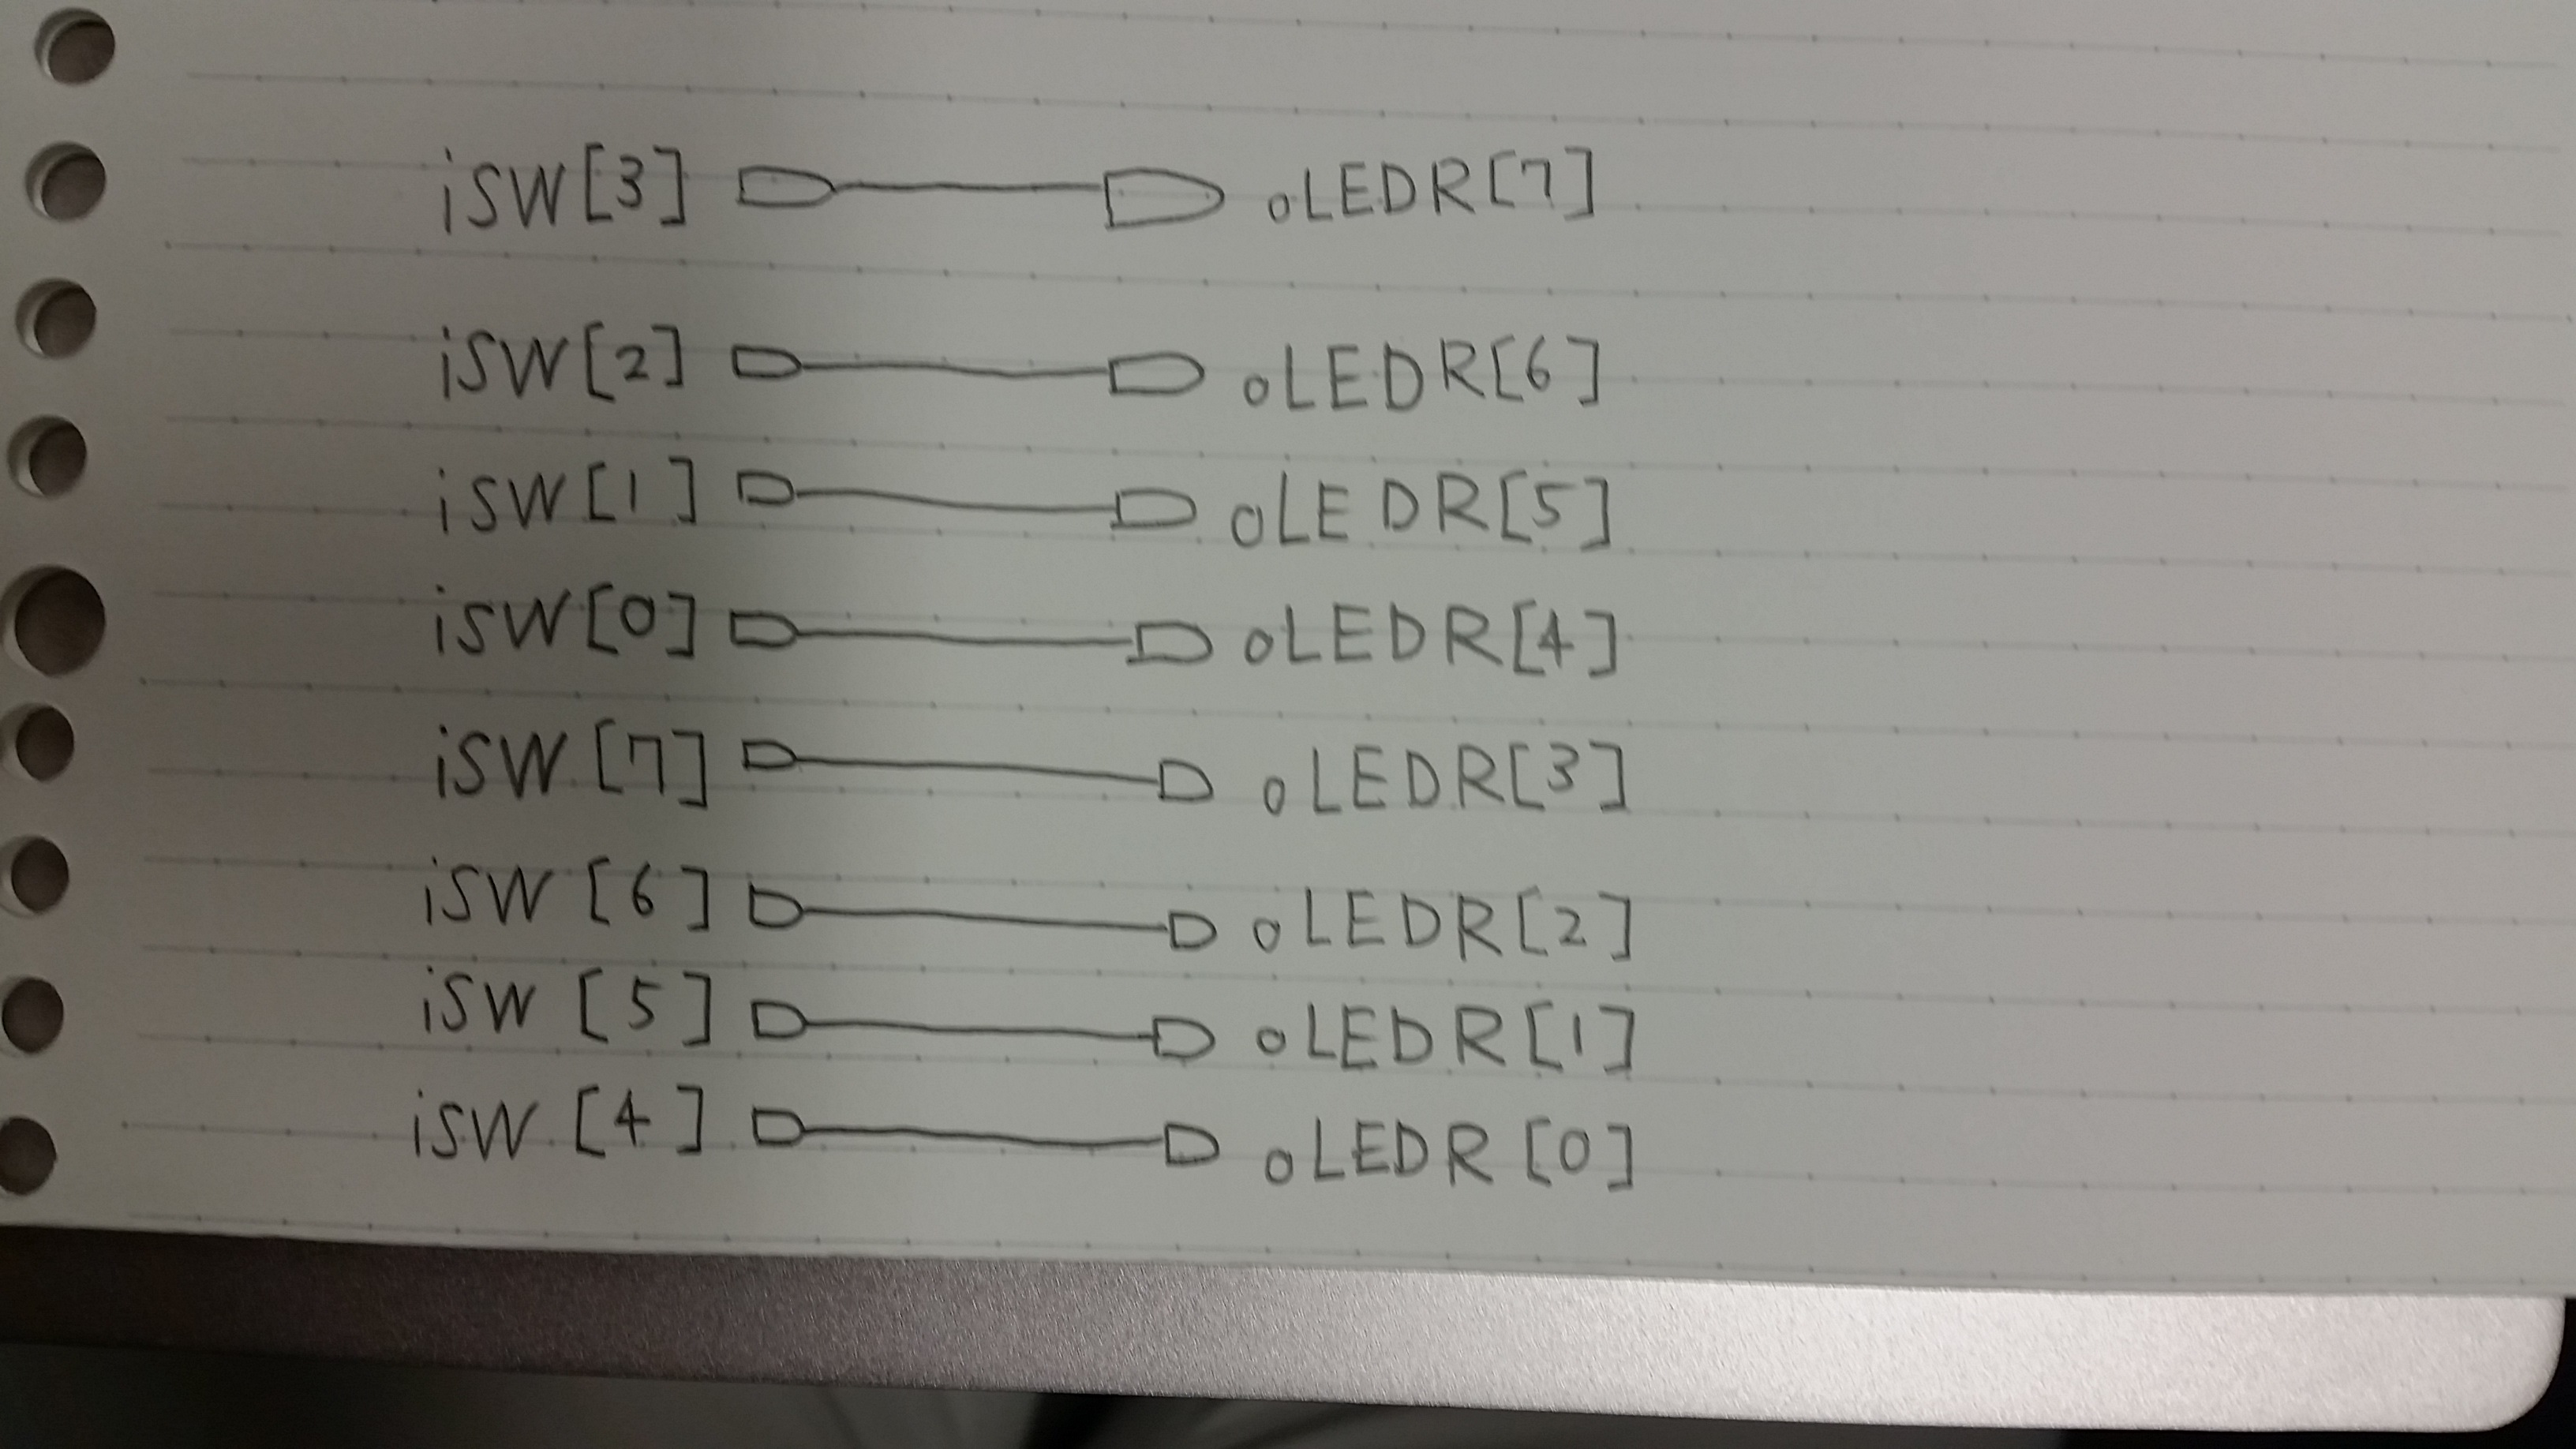
\includegraphics[width=15cm]{work6/CircuitDiagram.jpg}
\subsubsection{考察}
一つの配列に複数の配列をつなげる方法を知ったが、どの配線がどの配線と繋がっているかのわかりやすさという点では、下の二行のように分けて書く方がよいと感じた。
\subsection{課題7}
\subsubsection{目的}
全加算器のプロジェクトの中で、モジュール$halfadder$と$fulladder$を使って2ビットの加算器を$adder2.sv$として作成し、これをトップモジュールの中で使うようにし、スイッチや$LED$を使って試す。
\subsubsection{道のり}
まず、課題4で作成したモジュール$halfadder$と、課題5で作成した$fulladder$を使って、以下の画像のようにモジュール$adder2$を作成した。\\
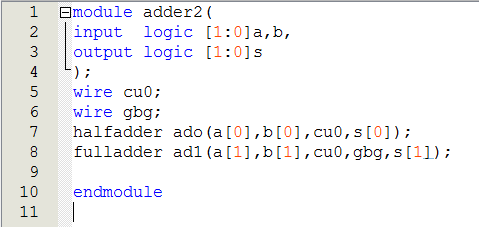
\includegraphics[width=10cm]{work7/7-4.PNG}\\
次に、以下の画像のように$adder2$をトップモジュールに組み込んだ。\\
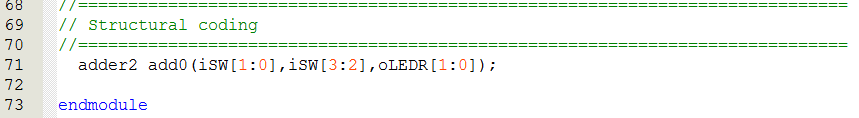
\includegraphics[width=15cm]{work7/7-1.PNG}\\
最後に、プロジェクトに半加算器、全加算器のソースコードと、$adder2.sv$を追加して、コンパイルしてハードウェア上で動作を確認した。
\subsubsection{結果}
意図したとおりに、$iSW[1:0]$と$iSW[3:2]$の加算の結果が$oLEDR[1:0]$に表示された。
\subsubsection{考察}
半加算器と全加算器を組み合わせて、多ビットの加算器を作成することが出来た。多ビットの加算の回路はすでに知っていたが、実際に自分たちで実装してみることでより細かく理解することが出来た。
\subsection{課題8}
\subsubsection{目的}
\subsubsection{道のり}
\subsubsection{結果}
\subsubsection{考察}
\subsection{課題9}
\subsubsection{目的}
\subsubsection{道のり}
\subsubsection{結果}
\subsubsection{考察}
\subsection{課題10}
\subsubsection{目的}
8ビットの加算器を設計する。これには2つの方針が考えられる。1つ目は、8ビット加算器を4ビットの加算器のつなぎ合わせとして定義し、4ビットの加算器を2ビットの加算器のつなぎ合わせとして定義するというように設計する方針である。2つ目は、いきなり1ビットの全加算器を8つ用いて8ビットの全加算器を構成するという方針である。
\subsubsection{道のり}
ここでは、二つ目の方針を採用した。\\
まず、以下の画像のようにモジュール$adder8$を定義した。\\
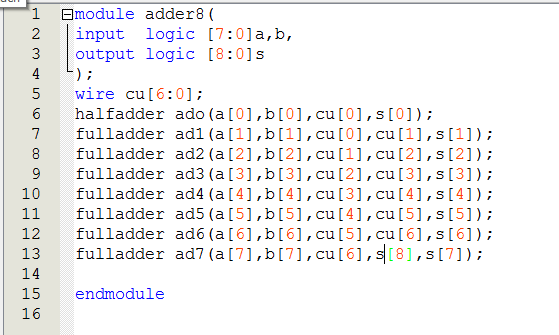
\includegraphics[width=10cm]{work10/10-2.PNG}\\
次に、以下の画像のようにモジュール$adder8$をトップモジュールに組み込んだ。\\
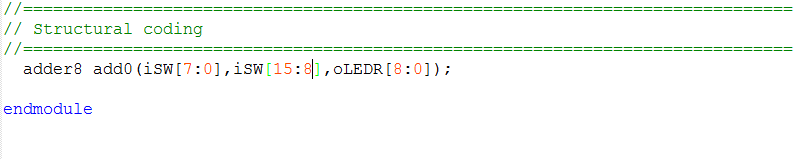
\includegraphics[width=15cm]{work10/10-1.PNG}\\
最後に、半加算器と全加算器のソースコードをプロジェクトに含め、コンパイルしてハードウェアに流し込み、動作を確認した。
\subsubsection{結果}
意図したとおりに、$iSW[7:0]$と$iSW[15:8]$の和が$oLEDR[7:0]$に表示された。
\subsubsection{考察}
ここでは二つ目の方針を採用した。課題7で2ビットの加算器を作成したが、二つ目の方針を採用した場合、入出力の大きさに応じて全加算器を追加することでより大きな加算器を作成することが出来ることが分かった。
\subsection{課題11}
\subsubsection{目的}
「+」演算子を使った動作モデル化による設計法を用いて、8ビット同士の加算を行うモジュールを定義し、スイッチなどを使って動作確認する。
\subsubsection{道のり}
ソースコード\ref{Work11TOP}のように、「+」演算子を使って$iSW \left[ 7:0 \right]$と$iSW \left[ 15:8 \right]$の和を$oLEDR \left[ 8:0 \right]$につなげ、コンパイルしてハードウェアに流し込み、動作を確認した。
\lstinputlisting[caption=$DE2_TOP.sv$,label=Work11TOP]{work11/DE2_TOP.sv}
\subsubsection{結果}
$oLEDR \left[ 8:0 \right]$は、正しく$iSW \left[ 7:0 \right]$と$iSW \left[ 15:8 \right]$の和を表していた。
\subsubsection{考察}
「+」演算子を使ったモジュールを定義し、動作を確認することで、$Verilog$の「+」演算子は、プログラミング言語の加算と同等の意味を持つことが分かった。また、この演算子の出力は、入力よりも1ビット大きく出力されることが分かった。ハードウェア記述言語でこのような演算子が定義されていることによって、回路の設計がより楽になるだろうと感じた。
\subsection{課題12}
\subsubsection{目的}
8ビットの2の補数表示の符号付き2進数どうしを加算して、9ビットの結果を得るモジュール$adder89$を定義し、スイッチなどを使って試す。
\subsubsection{道のり}
課題5で作成したモジュール$fulladder$を使って、モジュール$adder89$を以下のソースコード\ref{Work12Adder}のように作成した。
\lstinputlisting[caption=$adder89.sv$,label=Work12Adder]{work12/adder89.sv}
その後、以下のソースコード\ref{Work12TOP}のように$adder89$をトップモジュールに組み込んで、これをコンパイルし、ハードウェアに流し込んで動作を確認した。
\lstinputlisting[caption=$DE2\_TOP.sv$,label=Work12TOP]{work12/DE2_TOP.sv}
\subsubsection{結果}
意図したとおりに、二つの8ビットの入力$iSW[7:0],iSW[15:0]$の9ビットの和が、$oLEDR[8:0]$に表示された。
\subsubsection{考察}
課題5で作成したモジュール$fulladder$を複数組み合わせることによって、多ビットの加算を実現する回路を作成することが出来た。単純なものを組み合わせて複雑で大きなものを作っていくという点ではC言語などのプログラミング言語に似ていると感じた。プログラミングと同じような感覚ではーをウェアを設計できるようにすることで、設計の効率化を図ったのだろうと思った。
\subsection{課題13}
\subsubsection{目的}
\subsubsection{道のり}
\subsubsection{結果}
\subsubsection{考察}
\subsection{課題14}
\subsubsection{目的}
ソースコード\ref{Work14UnfixedModule}にあるリセットとイネーブルの入力(en)と繰り上がり出力(co)がついた10進カウンタの記述の$<$考えてね$>$の部分を補完し完成させて、組み込んで、キーボタンやLED等を使って動作を確認する。
\begin{lstlisting}[caption=count4.sv,label=Work14UnfixedModule]
//count4.svの中身(3/3)
//リセットとイネーブル付き10進カウンタ
module count4dre (
	input logic clk,
	input logic en,		//イネーブル
	input logic clr,	//クリア
	output logic [3:0] q,
	output logic co );	//繰り上がり
	// q == 9 のとき 1
	assign co = (q == 9) & en;
	always_ff @ (posedge clk) begin
		if (clk)	<考えてね>;
		else if (co)	<考えてね>;
		else id (en)	<考えてね>;
	end
endmodule
\end{lstlisting}
\subsubsection{道のり}
まず、ソースコード\ref{Work14UnfixedModule}を修正したソースコード\ref{Work14FixedModule}を用意し、それをソースコード\ref{Work14TOP}のようにトップモジュールに組み込み、コンパイルしてハードウェアに流し込み動作を確認した。
\lstinputlisting[caption=$count4.sv$,label=Work14FixedModule]{work14/count4.sv}
\lstinputlisting[caption=$DE2\_TOP.sv$,label=Work14TOP]{work14/DE2_TOP.sv}
\subsubsection{結果}
実際のハードウェア上では、次の状態遷移表\ref{Work14StateTransitionTable}のように動作した。リセットとイネーブル付き10進カウンタとして正しく動作した。
\begin{table}[!h]
	\begin{center}
		\caption{カウンタの状態遷移表}
		\label{Work14StateTransitionTable}
		\begin{tabular}{|c||c|c|c|c|}
			\hline
			\backslashbox{現状態\\($q$の値)}{$\left(en,clr\right)$}	&$\left(0,0\right)$	&$\left(0,1\right)$	&$\left(1,0\right)$	&$\left(1,1\right)$\\	\hline
			$0$							&$0$			&$0$			&$1$			&$0$\\			\hline
			$1$							&$1$			&$0$			&$2$			&$0$\\			\hline
			$2$							&$2$			&$0$			&$3$			&$0$\\			\hline
			$3$							&$3$			&$0$			&$4$			&$0$\\			\hline
			$4$							&$4$			&$0$			&$5$			&$0$\\			\hline
			$5$							&$5$			&$0$			&$6$			&$0$\\			\hline
			$6$							&$6$			&$0$			&$7$			&$0$\\			\hline
			$7$							&$7$			&$0$			&$8$			&$0$\\			\hline
			$8$							&$8$			&$0$			&$9$			&$0$\\			\hline
			$9$							&$9$			&$0$			&$0$			&$0$\\			\hline
		\end{tabular}
	\end{center}
\end{table}
\subsubsection{考察}
問題文にあるソースコードを修正して、目的のカウンタを作った。ModelSimで波形を確認したところ、正しい波形を得ることが出来たが、ハードウェア上では正しく動作させることが出来なかった。ソースコード\ref{Work14Testbench}はModelSimで使用したテストベンチである。
\lstinputlisting[caption=$testbench.sv$,label=Work14Testbench]{work14/testbench.sv}
\subsection{課題15}
\subsubsection{目的}
$oHEX[6:0]$にスイッチ$iSW[6:0]$をつないで、日の字型のどの部分に対応しているのかを調べて、結果を表にまとめる。
\subsubsection{道のり}
\subsubsection{結果}
\subsubsection{考察}
\subsection{課題16}
\subsubsection{目的}
\subsubsection{道のり}
\subsubsection{結果}
\subsubsection{考察}
\subsection{課題17}
\subsubsection{目的}
0以上9以下の4ビットの入力を受け取り、日の字型LED($oHEX0\_D\left[6:0\right]$)にその値を表示するためのモジュールを作成する。その際、以下のalways文を使ったソースコード\ref{Work17UnfixedModuleAlwaysVer}またはfunction文を使ったソースコード\ref{Work17UnfixedModuleFunctionVer}を修正して目的のモジュールを作成する。
\begin{lstlisting}[caption=always文版,label=Work17UnfixedModuleAlwaysVer]
module	deg7dec (
	input	logic	[3:0]	bdc,
	output	logic	[6:0]	seg);

	always_comb
		case	(bdc)
			4'b0000:	seg = 7'b0のパターン;
			4'b0001:	seg = 7'b1のパターン;
			4'b0010:	seg = 7'b1111111;//これウソ
			.....
			default:	seg = 7'b1111111;//全部消灯
		endcase
endmodule
\end{lstlisting}
\begin{lstlisting}[caption=function文版,label=Work17UnfixedModuleFunctionVer]
module deg7dec (
	input	logic	[3:0]	bdc,
	output	logic	[6:0]	seg);

	assign seg = b7s(bdc);

	function [6:0] b7s;
		input	[3:0]	bdc;
		case	(bdc)
			4'b0000:	b7s = 7'b0に対応するパターン;
		endcase
endmodule
\end{lstlisting}
\subsubsection{道のり}
まず、上のソースコード\ref{Work17UnfixedModuleAlwaysVer}とソースコード\ref{Work17UnfixedModuleFunctionVer}を修正して、それぞれ以下のソースコード\ref{Work17FixedModuleAlwaysVer}とソースコード\ref{Work17FixedModuleFunctionVer}を作成した。
\lstinputlisting[caption=$always.sv$,label=Work17FixedModuleAlwaysVer]{work17/always.sv}
\lstinputlisting[caption=$function.sv$,label=Work17FixedModuleFunctionVer]{work17/function.sv}
その後、トップモジュールを以下のソースコード\ref{Work17TOP}のように作成して、ソースコード\ref{Work17FixedModuleAlwaysVer}とソースコード\ref{Work17TOP}を含むプロジェクトと、ソースコード\ref{Work17FixedModuleFunctionVer}とソースコード\ref{Work17TOP}を含むプロジェクトを作成し、それぞれコンパイルしてハードウェアに流し込み動作を確認した。
\lstinputlisting[caption=$DE2\_TOP.sv$,label=Work17TOP]{work17/DE2_TOP.sv}
\subsubsection{結果}
実際のハードウェア上での動作は、どちらのソースコードを用いても以下の真理値表に従い、0から9までの数字を正しく表示していた。
\begin{table}[!h]
	\begin{center}
		\caption{課題17の結果の真理値表}
		\label{Work17TruthTable}
		\begin{tabular}{|c|c|c|c||c|c|c|c|c|c|c|}
			\hline
			\multicolumn{4}{|c|}{$iSW \left[ 3:0 \right]$}							&\multicolumn{7}{|c|}{$oHEX0\_D \left[ 6:0 \right]$}															\\	\hline
			$\left[ 3 \right]$	&$\left[ 2 \right]$	&$\left[ 1 \right]$	&$\left[ 0 \right]$	&$\left[ 0 \right]$	&$\left[ 1 \right]$	&$\left[ 2 \right]$	&$\left[ 3 \right]$	&$\left[ 4 \right]$	&$\left[ 5 \right]$	&$\left[ 6 \right]$	\\	\hline\hline
			$0$			&$0$			&$0$			&$0$			&$0$			&$0$			&$0$			&$0$			&$0$			&$0$			&$1$			\\	\hline
			$0$			&$0$			&$0$			&$1$			&$1$			&$0$			&$0$			&$1$			&$1$			&$1$			&$1$			\\	\hline
			$0$			&$0$			&$1$			&$0$			&$0$			&$0$			&$1$			&$0$			&$0$			&$1$			&$0$			\\	\hline
			$0$			&$0$			&$1$			&$1$			&$0$			&$0$			&$0$			&$0$			&$1$			&$1$			&$0$			\\	\hline
			$0$			&$1$			&$0$			&$0$			&$1$			&$0$			&$0$			&$1$			&$1$			&$0$			&$0$			\\	\hline
			$0$			&$1$			&$0$			&$1$			&$0$			&$1$			&$0$			&$0$			&$1$			&$0$			&$0$			\\	\hline
			$0$			&$1$			&$1$			&$0$			&$0$			&$1$			&$0$			&$0$			&$0$			&$0$			&$0$			\\	\hline
			$0$			&$1$			&$1$			&$1$			&$0$			&$0$			&$0$			&$1$			&$1$			&$0$			&$1$			\\	\hline
			$1$			&$0$			&$0$			&$0$			&$0$			&$0$			&$0$			&$0$			&$0$			&$0$			&$0$			\\	\hline
			$1$			&$0$			&$0$			&$1$			&$0$			&$0$			&$0$			&$0$			&$1$			&$0$			&$0$			\\	\hline
			$1$			&$0$			&$1$			&$0$			&$1$			&$1$			&$1$			&$1$			&$1$			&$1$			&$1$			\\	\hline
			$1$			&$0$			&$1$			&$1$			&$1$			&$1$			&$1$			&$1$			&$1$			&$1$			&$1$			\\	\hline
			$1$			&$1$			&$0$			&$0$			&$1$			&$1$			&$1$			&$1$			&$1$			&$1$			&$1$			\\	\hline
			$1$			&$1$			&$0$			&$1$			&$1$			&$1$			&$1$			&$1$			&$1$			&$1$			&$1$			\\	\hline
			$1$			&$1$			&$1$			&$0$			&$1$			&$1$			&$1$			&$1$			&$1$			&$1$			&$1$			\\	\hline
			$1$			&$1$			&$1$			&$1$			&$1$			&$1$			&$1$			&$1$			&$1$			&$1$			&$1$			\\	\hline
		\end{tabular}
	\end{center}
\end{table}
\subsubsection{考察}
日の字型LEDで数字を表示するという同じ働きをする二つのモジュールを作成し、それぞれ同一のトップモジュールに組み込んで動作を確認した。数字をひとつ表示するだけでも、かなり大きなデコーダの真理値表を基にして作ったので大変だった。日の字型LEDではなく、普通のディスプレイのような小さな画素の二次元配列上に文字を表示させるのはもっと大変なのだろうと感じた。
\subsection{課題18}
\subsubsection{目的}
\subsubsection{道のり}
\subsubsection{結果}
\subsubsection{考察}
\subsection{課題19}
\subsubsection{目的}
\subsubsection{道のり}
\subsubsection{結果}
\subsubsection{考察}
\subsection{課題20}
\subsubsection{目的}
\subsubsection{道のり}
\subsubsection{結果}
\subsubsection{考察}
\section{実験の総括的なまとめや感想}
\end{document}
